\section{Versuchsaufbau und Durchf\"uhrung}
\subsection{Versuchsaufbau}
In diesem Versuch soll die Photolumineszenz von Quantenpunkten gemessen werden. Die dafür notwendigen Apparate sind in dem Kapitel \ref{sec:Grundlagen} beschrieben. 
Die wichtigsten Bauteile sind ein He-Ne-Laser zur Anregung der Quentenpunkte, die Quantenpunkte selber und ein Spektrometer zur Messung des Spektrums. 
Die Temperatur hat, wie im Kapitel \ref{sec:Grundlagen} beschrieben einen großen Einfluss auf das Spektrum. 
Zur Einstellung der benötigten Temperaturen wird ein Helium Kryostat benutzt, wodurch Temperaturen bis $4$ K erreicht werden können. 
Der schematische Versuchaufbau ist in der Abbildung \ref{fig:Versuchsaufbau} dargestellt.  
\begin{figure}[H]
\centering
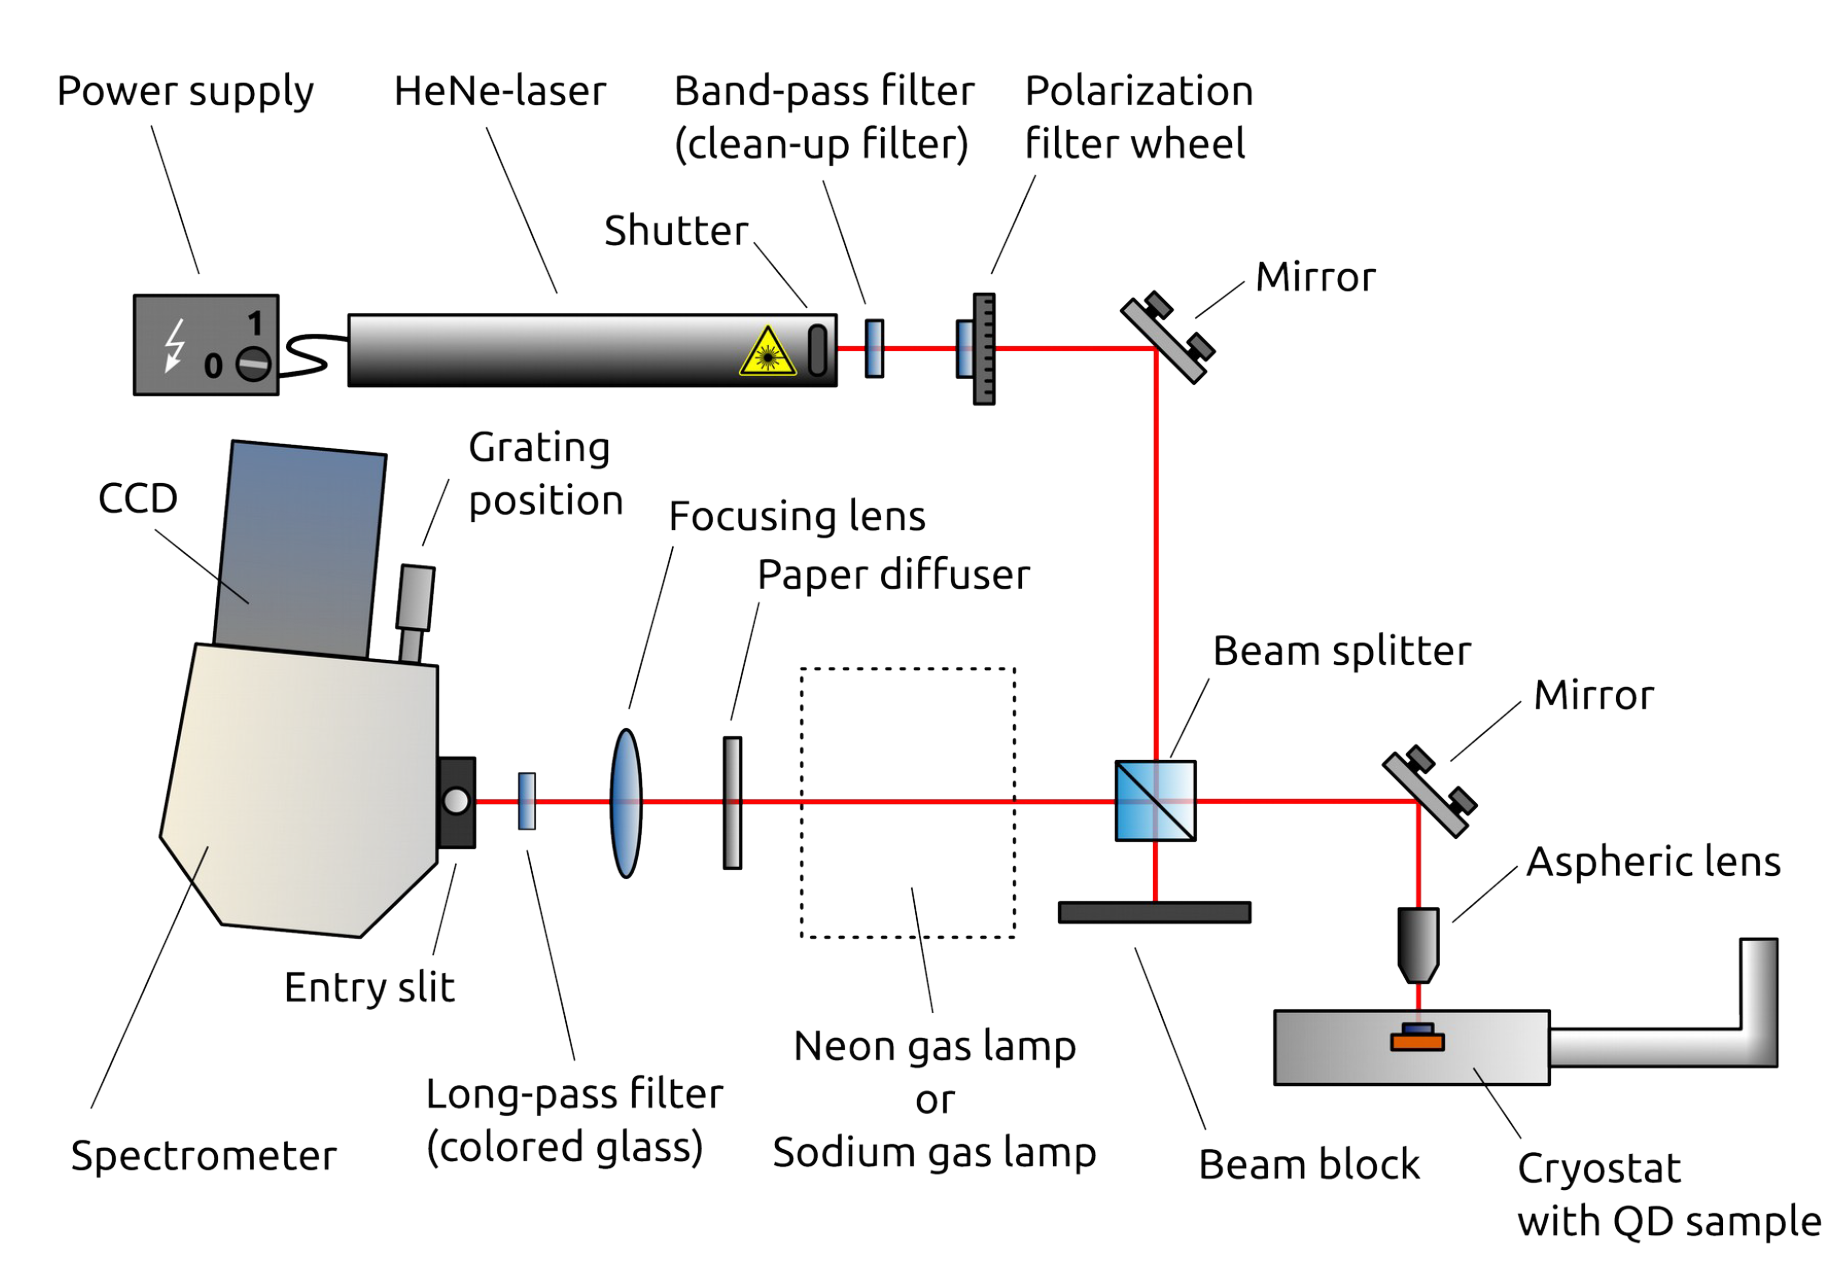
\includegraphics[scale=0.2]{versuchsaufbau.PNG}
\caption{Schematischer Versuchsaufbau zur Messung der Photolumineszenz von Quantenpunkten \cite{anleitung}.   }
\label{fig:Versuchsaufbau}
\end{figure}
\subsection{Spektrometer}
Die Messung mit dem Spektrometer wird von einem Computer aus gesteuert. Das Rauschen in dem Spektrum kann durch eine Abkühlung des Detektors auf $-45\ {}^\circ\mathrm{C}$ reduziert werden. Zur Kühlung wird ein Peltier-Element verwendet. 
Die Aufnahme-Parameter für die Messungen, wie zum Beispiel die Integrationszeit, können in der Spektrometer-Software selber engestellt werden. 
Desweiteren kann die Signalqualität auch durch das Entferenen des Dunkelrauschen verbessert werden. 
Dazu wird das Spektrometer Licht-dicht abgedeckt und dann das Dunkelspektrum gemessen. 
Dieses kann dann automatisch von den gemessenen Spektren abgezogen werden. 
Durch die Abhängigkeit des Dunkelspektrums von der Integrationszeit muss nach jedem Wechsel der Integrationszeit das Dunkelspektrum neu gemessen werden. 
Zu beachten bei der Verwendung des Spektrometers ist, das die CCD-Kamera nicht gesättigt werden darf, da dies zu schäden an der Kamera führen kann. 
Außerdem muss die Belichtungszeit der Lichtquelle angepasst werden, um die Qualität des Spektrums zu verbessern. 
Um die korrekte Funktionsweise des Spektrometers zu testen, soll vor den eigentlichen Messungen das Spektrum einer anderen Quelle, zum Beispiel der Raumbeleuchtung, gemessen werden. 
Dabei kann untersucht werden, inwiefern Streulicht vorhanden ist und wie es gegebenenfalls reduziert werden kann. 
\subsection{Spektrale Kalibrierung des Spektrometers}
\label{sec:Kalibrierung}
Das Gitter in dem Spektrometer muss vor jeder Messung auf den benötigten Wellenlängenbereich eingestellt werden. 
Dazu kann mit einer Mikrometerschraube am Spektrometer die Zentralwellenlänge eingestellt werden. 
Diese Zentralwellenlänge muss auch in der Spektrometer-Software eingegeben werden. 
Diese manuelle Einstellung der Zentralwellenlänge kann nicht exakt durchgeführt werden. 
Deshalb ist eine spektrale Kalibrierung des Spektrometers notwendig.
Dazu wird eine Neon-Dampflampe auf der optischen Achse vor dem Spektrometer plaziert. Durch die Verwendung einer Papier-Streuscheibe kann eine diffuse Beleuchtung realisiert werden.
Eine weiter Mikrometerschraube kann die Spaltbreite am Spektrometer einstelln. Dabei muss beachtet werden, das selbst bei einer  Spaltbreite von $0\ \mu$m der Spalt nicht ganz geschlossen ist. 
Es kommt immer noch soviel Licht durch, das die Kalibrierung bei geschlossem Spalt durchgeführt werden kann.
Für die eigentliche Kalibrierung muss die Zentralwellenlänge für Neon eingestellt werden. 
Das damit aufgenommene Spektrum soll nun mit dem zu erwartetem Spektrum verglichen werden. 
Die Spektrometer-Software muss nun so kalibriert werden, dass die gemessenen Emissionslinien mit den erwarteten übereinstimmen. 
\subsection{Auflösungsvermögen des Spektrometers}
Im zweitem Versuchsteil soll das Auflösungsvermögen \eqref{eq:Auflösung} des Spektrometers bestimmt werden. 
Die Auflösung hängt von der Spaltbreite am Eingang zum Spektrometer ab. Der Einfluss der Spaltbreite soll in diesem Versuchsteil analysiert werden. 
Dazu wird eine Natrium-Dampflampe auf der optische Achse vor dem Spektrometer plaziert. 
Analog zu der Neon-Dampflampe in Kapitel \ref{sec:Kalibrierung} soll mittels einer Papier-Streuscheibe eine diffuse Beleuchtung des Spektrometers gewält werden. 
Für mindestens $10$ Eingangsspaltbreiten aus dem Bereich $0\ \mu\mathrm{m} - 600\ \mu\mathrm{m}$ soll das Spektrum des NA(I)-Doubletts gemessen werden. 
Wie bereits im Kapitel \ref{sec:Kalibrierung} muss beachtet werden, dass eine an der Mikrometerschraube eingestellte Spaltbreite von $0\ \mu$m nicht bedeutet, dass der Eingangsspalt tatsächlich geschlossen ist.
Das Auflösungsvermögen soll nach Gleichung \eqref{eq:Auflösung} bestimmt werden.

\subsection{Vorjustage des Photolumineszenzaufbaus}
\label{sec:Justage}
Nach der Analyse des Spektrometers in den beiden vorherigen Versuchsteilen soll nun das eigentliche Experiment, die Messung der Photolumineszenz von Quantenpunkten, durchgeführt werden. 
Als erstes muss mit dem Kryostaten die Temperatur auf ca. $4$ K reduziert werden. 
Danach kann die Vorjustage des Photolumineszenzaufbaus durchgeführt werden. 
Dabei ist zu beachten, dass der Laser eine Ausgangsleistung von $30$ mW im sichtbaren Spektralbereich hat. 
Direkter oder indirekter Einfall in das menschliche Auge muss deshalb vermieden werden. 
Die Leistung des Lasers, kann mit einem Polarisator eingestellt werden. 
Zur Vorjustage muss durch verstellen der Spiegel versucht werden, dass der Laserstrahl möglichst senkrecht auf die Probe trifft. 
Dabei ist die Rückreflexion zu beachten.
Außerdem muss der reflektierte Laserstrahl auch noch auf den Spektrometer treffen. 
Als nächstes können die Linsen in den Versuchsaufbau eingesetzt werden. 
Die Justierung muss nun erneut, nach den bereits genannten Kriterien, verbessert werden. 
Durch Veränderung der Position der Linse in dem Strahlgang kann der Laser möglichst gut auf den Spektrometer fokussiert werden. 
\subsection{Photolumineszenzmessung}
Nach der Justage der optischen Bauteile, siehe Kapitel \ref{sec:Justage}, kann mit der Messung begonnen werden.
Dazu muss der richtige Zentralwellenlängebereich eingestellt werden, siehe Kapitel \ref{sec:Kalibrierung}. 
Die Temperatur der Probe soll bei ca. $4$ K liegen. Für unterschiedliche Anregungsleistungen soll nun das Spektrum gemessen werden.  
Zusätzlich soll auch die Messung der Temperaturabhängigkeit der Photolumineszenzmessung untersucht werden. 
Dazu wird mittels einer Heizspannung und der Reduzierung der Heliumzufuhr zur Kühlung die Temperatur variiert werden.
In Schritten von ca. $20$ K soll die Temperatur erhöht werden, bis nur noch ein Peak in dem Spektrum sichtbar. Die Ursache für das verschwinden der Peaks ist in dem Kapitel \ref{sec:Grundlagen} erläutert. 
Diese beiden Messungen sollen für 2 unterschiedliche Quantenpunkte gemacht werden. 
Nach dem Wechsel der Probe ist eine neue Justierung, siehe Kapitel \ref{sec:Justage}, durchzuführen.  


